% the Dirichlet condition by row replacement
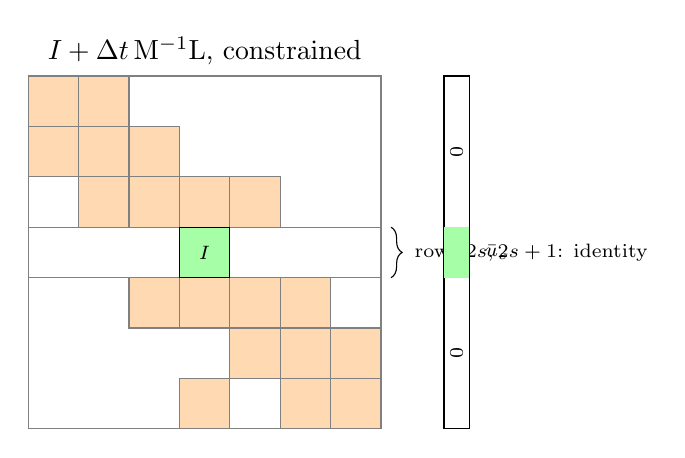
\begin{tikzpicture}[scale=0.32]
  \draw[gray] (0,0) rectangle (14,-14);
  \foreach \i/\j in {0/0,0/2,2/0,2/2,2/4,4/2,4/4,4/8,8/4,8/8,8/10,10/8,10/10,10/12,12/10,12/12,6/6,6/4,4/6,6/8,8/6,6/12,12/6}
    \filldraw[draw=gray, fill=orange!30] (\j,-\i) rectangle ++(2,-2);
  \fill[white] (0,-6) rectangle (14,-8);
  \draw[gray] (0,-6) rectangle (14,-8);
  \filldraw[draw=black, fill=green!35] (6,-6) rectangle ++(2,-2);
  \node[font=\scriptsize] at (7,-7) {$I$};
  \draw[decorate, decoration={brace, amplitude=4pt}] (14.4,-6) -- (14.4,-8) node[midway, right=5pt, font=\scriptsize, align=left] {rows $2s, 2s+1$: identity};
  \draw (16.5,0) rectangle (17.5,-14);
  \fill[green!35] (16.5,-6) rectangle (17.5,-8);
  \node[font=\scriptsize, rotate=90] at (17,-3) {$0$};
  \node[font=\scriptsize, rotate=90] at (17,-11) {$0$};
  \node[font=\scriptsize] at (18.6,-7) {$\bar u_s$};
  \node at (7,1) {$I + \Delta t\, \mathrm M^{-1} \mathrm L$, constrained};
\end{tikzpicture}
